\chapter{Конструкторский раздел}
STOOPED HERE!
В данном разделе представлены схемы алгоритмов работы главного потока и конвейера.

\section{Схемы алгоритмов}
Схема алгоритма работы главного потока представлена  на рисунке \ref{ZBufferAlg}.
Схема алгоритма работы ленты конвейера представлена  на рисунке \ref{ZBufferWithThreads}. Здесь представлен общий вид схемы, а под обработкой заявки понимаются разные алгоритмы. Лента 1 выполняет алгоритм, представленный на рис. \ref{getWords}, лента 2 -- алгоритм, представленный на рис. \ref{getPolinoms}, лента 3 -- алгоритм, представленный на рис. \ref{getLongestPolinom}.  

\begin{figure}
	\center{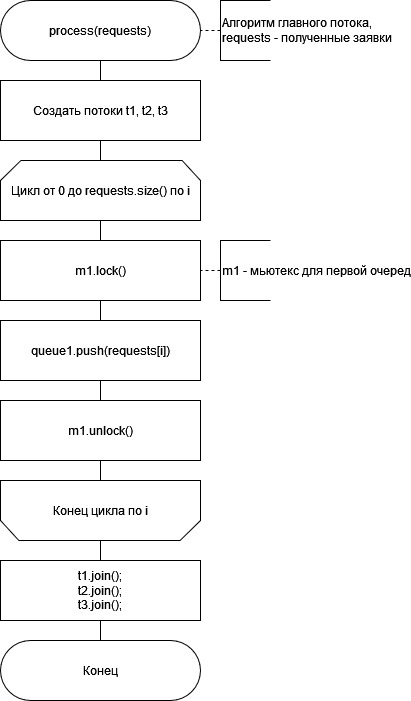
\includegraphics[width=0.8\linewidth]{inc/img/MainThread}}
	\caption{Схема алгоритма работы главного потока}
	\label{ZBufferAlg}
\end{figure}

\begin{figure}
	\center{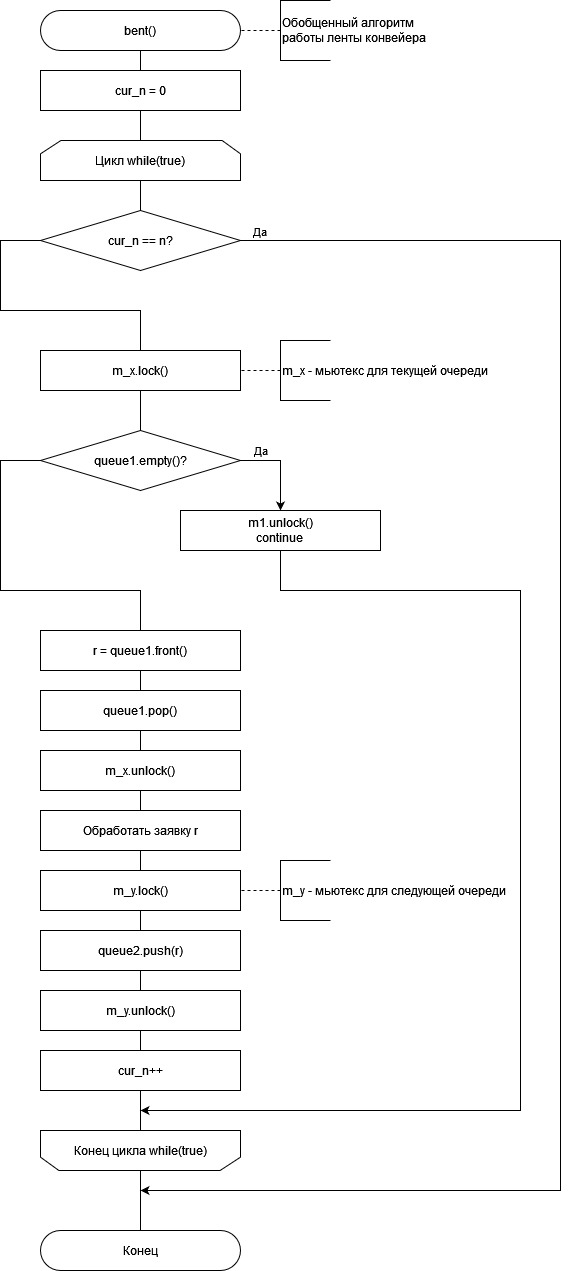
\includegraphics[width=0.7\linewidth]{inc/img/Conveer}}
	\caption{Обобщенная схема алгоритма работы ленты конвейера}
	\label{ZBufferWithThreads}
\end{figure}

\begin{figure}
	\center{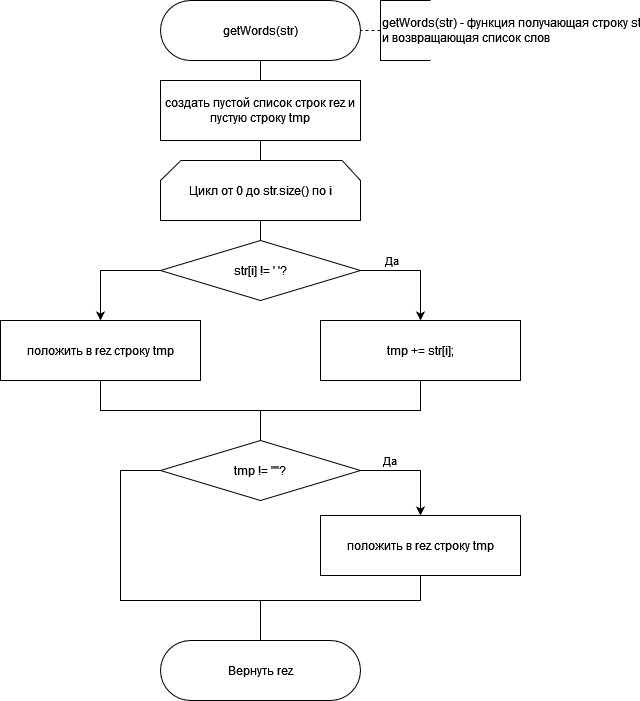
\includegraphics[width=1\linewidth]{inc/img/getWords}}
	\caption{Схема алгоритма разбиения строки на слова}
	\label{getWords}
\end{figure}

\begin{figure}
	\center{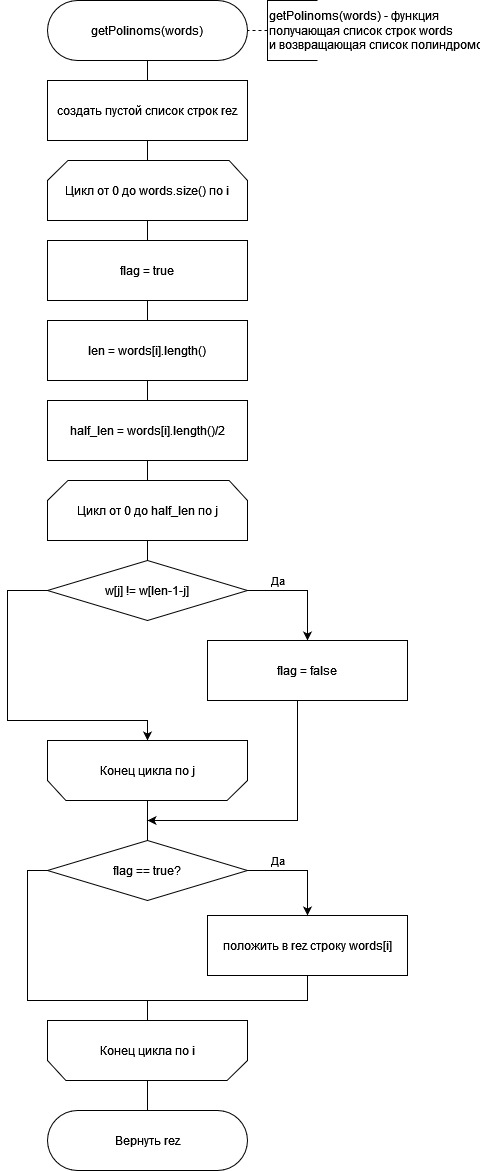
\includegraphics[width=0.6\linewidth]{inc/img/getPolinoms}}
	\caption{Схема алгоритма нахождения всех полиндромов из полученных слов}
	\label{getPolinoms}
\end{figure}

\begin{figure}
	\center{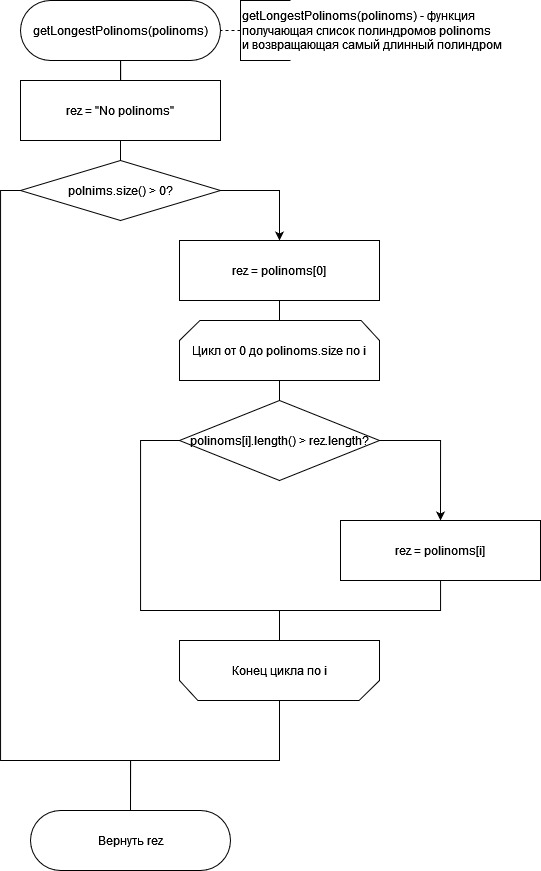
\includegraphics[width=0.9\linewidth]{inc/img/getLongestPolinom}}
	\caption{Схема алгоритма самого длинного полиндрома}
	\label{getLongestPolinom}
\end{figure}

\newpage
\section{Вывод}
В данном разделе были разработаны схемы алгоритмов работы главного потока, обобщенная схема алгоритма работы ленты конвейера и схемы алгоритмов обработки заявок.